\documentclass{article}
\usepackage{xeCJK}
\usepackage{tikz}
\usepackage{graphics}

\begin{document}
\title{第一章:线}
\author{刘邦}
\maketitle
\newpage

\section{绘制直线}
\begin{figure}[htp]
    \centering
    \begin{tikzpicture}[>=latex]
        % 坐标起始位置
        \draw[<->] (0, 0) -- (5, 0);
        \draw[->] (0, -1) -- (5, -1);
        \draw[<-] (0, -2) -- (5, -2);
        \draw[|<-] (0, -3) -- (5, -3);
        \draw[->|] (0, -4) -- (5, -4);
        \draw[|<->|] (0, -5) -- (5, -5);
    \end{tikzpicture}
    \caption{lines latex}
\end{figure}

\begin{figure}[htp]
    \centering
    \begin{tikzpicture}[>=stealth]
        % 坐标起始位置
        \draw[<->, dashed, thick] (0, 0) -- (5, 0);
        \draw[->, dotted, very thick] (0, -1) -- (5, -1);
        \draw[<-, dashdotted, ultra thick] (0, -2) -- (5, -2);
        \draw[|<-, thin] (0, -3) -- (5, -3);
        \draw[->|, very thin] (0, -4) -- (5, -4);
        \draw[|<->|, ultra thin] (0, -5) to (5, -5);
        \draw[dashed] (0, -6) -- (5, -6);
        \draw[dotted] (0, -7) -- (5, -7);
        \draw[dashdotted] (0, -8) -- (5, -8);
    \end{tikzpicture}
    \caption{lines stealth}
\end{figure}

\begin{figure}[htp]
    \centering
    \begin{tikzpicture}
        \draw[thick] (0, 0) node[below]{直线下方} -- (5, 0);
        \draw[thick] (0, -1) -- (5, -1) node[above]{直线上方};
        \draw[|<->|] (0, -2) -- node[fill=white]{直线中间} (5, -2);
        % 20%红色和80%白色调配填充
        \draw[|<->|] (0, -3) -- node[fill=red!20!white]{直线中间} (5, -3);
        \draw[|<->|] (0, -4) -- node[below]{直线下面} (5, -4);
    \end{tikzpicture}
    \caption{}
\end{figure}

\newpage
\section{绘制坐标系}
\begin{figure}[htp]
    \centering
    \begin{tikzpicture}[>=latex]
        \draw[->] (-1, 0) -- (4, 0)node[right]{$x$};
        \draw[->] (0, -1) -- (0, 4)node[right]{$y$};
        \draw (0, 2)node[left]{$N$} -- (2, 2)node[right]{$P(x, y)$} -- (2, 0)node[below]{$M$};
        \node at (-.2, -.2){$O$};
        % 画刻度值
        \draw(0, 1)node[left]{$1$} -- (.1, 1);
        \draw(1, 0)node[below]{$1$} -- (1, .1);
    \end{tikzpicture}
    \caption{}
\end{figure}

\begin{figure}[htp]
    \centering
    \begin{tikzpicture}[>=latex]
        \draw[->] (-1, 0) -- (4, 0)node[right]{$x$};
        \draw[->] (0, -1) -- (0, 4)node[right]{$y$};
        \node at (-.2, -.2){$O$};

        % 通过foreach自动绘制刻度
        \foreach \x in {1, 2, ..., 6}
            {
                \draw (0, \x*0.5)node[left]{$\x$} -- (.1, \x*0.5);
                \draw (\x*0.5, 0)node[below]{$\x$} -- (\x*0.5, .1);
            }
    \end{tikzpicture}
    \caption{}
\end{figure}

\newpage
\section{填充颜色}

\begin{figure}[htp]
    \centering
    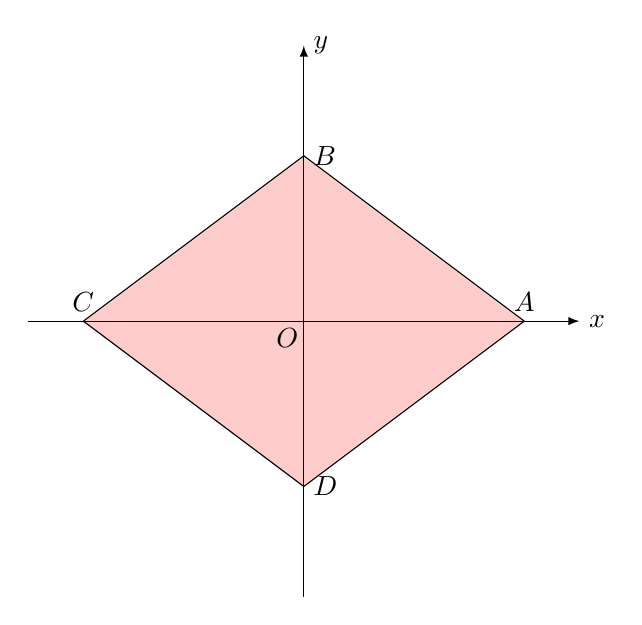
\begin{tikzpicture}[>=latex, scale=.7]
        \draw[fill=red!20!white] (-4, 0)node[above]{$C$} -- (0, 3)node[right]{$B$} -- (4, 0)node[above]{$A$} -- (0, -3)node[right]{$D$} -- (-4, 0);
        \draw[->] (-5, 0) -- (5, 0)node[right]{$x$};
        \draw[->] (0, -5) -- (0, 5)node[right]{$y$};
        \node at (-.3, -.3){$O$};
    \end{tikzpicture}
    \caption{}
\end{figure}

\newpage
\section{绘制基本图形}

\begin{figure}[htp]
    \centering
    
\begin{tikzpicture}[>=latex]
        \draw[fill=cyan] (0, 0) rectangle (6, 4);
        \fill[cyan, draw=black] (0, -5) rectangle (6, -1);
        \fill[cyan] (0, -10) rectangle (6, -6);
    \end{tikzpicture}
    \caption{}
\end{figure}

\begin{figure}[htp]
    \centering
    
\begin{tikzpicture}[>=latex]
        \fill[cyan] (0, 0) circle (1.5);
    \end{tikzpicture}
    \caption{}
\end{figure}


\end{document}
